\section{Outlook}

\setbeamertemplate{frame footer}{\cite{Patel2015}}
\begin{frame}
    \frametitle{Abdominal Aortic Aneurysm (AAA) - Current Modelling Technique}
    \begin{columns}[onlytextwidth]
        \begin{column}{0.5\textwidth}
            \begin{itemize}
                \item Modelling from Aortic-Valve to Iliac-Bifurcation
                \item Modelling based on computer tomography (CT) or magnet resonance
                      imaging (MRI)
                \item Rigid walls (only fluid domain modelled)
                \item Transient boundary conditions derived from literature
                \item Newtonian fluid model
                \item Transient simulation
                \item Simulation with commercial and open source CFD packages.
            \end{itemize}
        \end{column}
        \begin{column}{0.5\textwidth}
            \begin{figure}[ht]
                \centering
                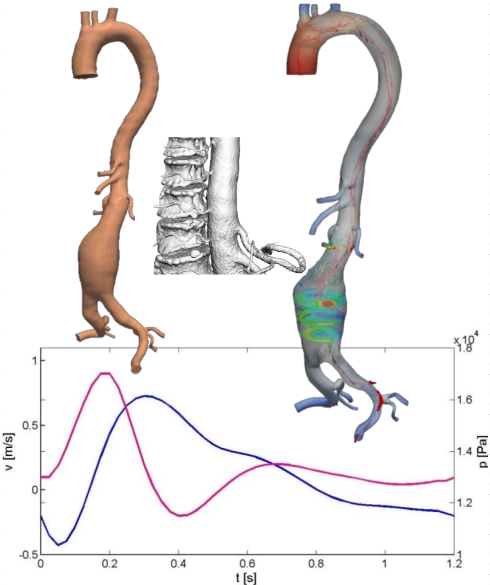
\includegraphics[width=0.7\textwidth]{aorta_current_modelling}
            \end{figure}
        \end{column}
    \end{columns}
\end{frame}
\begin{frame}
    \frametitle{Plans - Modelling FSI and cracking}
    Modelling of the FSI with non-Newtonian fluid (blood) and also modelling the crack
    propagation of the aorta due to AAA.
    \begin{columns}[onlytextwidth]
        \begin{column}{0.5\textwidth}
            \begin{figure}[ht]
                \centering
                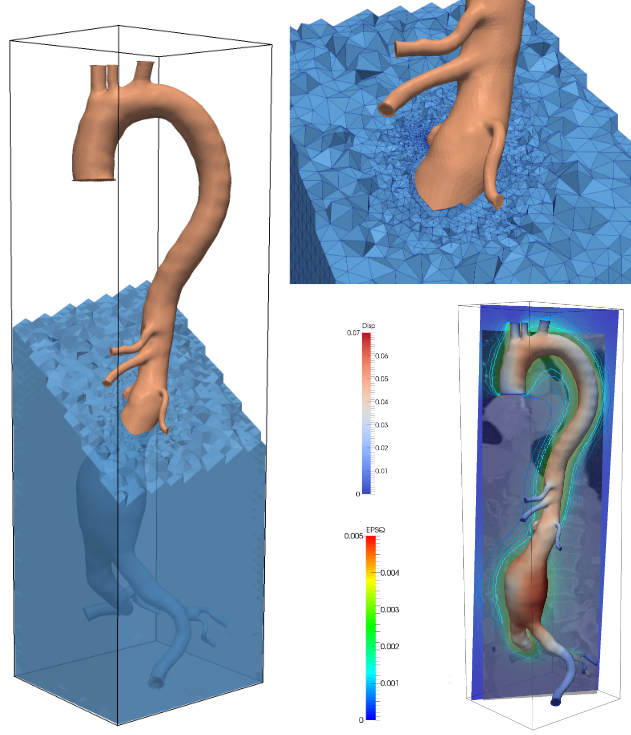
\includegraphics[width=0.6\textwidth]{aorta_fsi}
                \caption{Mesh-based approach - large scale problem}
            \end{figure}
        \end{column}
        \begin{column}{0.5\textwidth}
            \begin{figure}[ht]
                \centering
                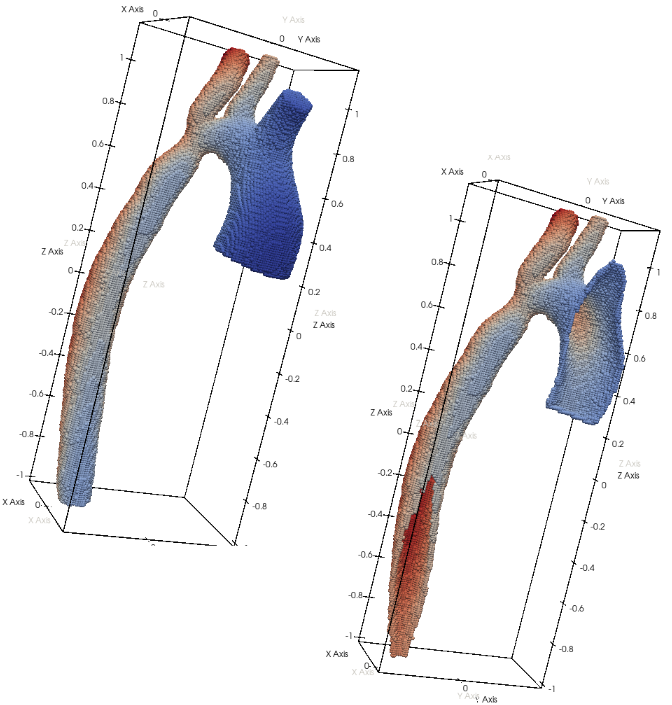
\includegraphics[width=0.7\textwidth]{aorta_particles}
                \caption{Particle-based approach - to be done with
                    \texttt{TrixiParticles.jl}}
            \end{figure}
        \end{column}
    \end{columns}
\end{frame}
\setbeamertemplate{frame footer}{}
